\documentclass[
                aspectratio=169, 
                14pt,
                % notes,
                % notes=only,
                ]{beamer}



\usepackage{../../Common/slidePreamble} % include your preamble.sty file


% Usage example
\title[Short Form Title]{
    Long Form Title
    }
% \subtitle{A Study Conducted in 2023}

\author[author 1 \and author 2]{ author 1 \and author 2}


\date{\footnotesize Host Of Conference\\ Anual General Meeting\\ \today}





\begin{document}

\begin{frame}[shrink=20]
    \titlepage
\end{frame}



% \begin{frame}[shrink=20]{Table Of Contents}

%     % \footnotesize
%     % \scriptsize
%     % \tiny
%     % \small
%     % \begin{multicols}{2}
%     \tableofcontents
%     % \end{multicols}

% \end{frame}

\begin{frame}[shrink=40]{Abbreviations \& Operational Definitions}

    % \footnotesize
    % \scriptsize
    % \tiny
    % \small
    \begin{multicols}{2}
    \printglossary[type=\acronymtype, title=Keywords]

    \printglossary[title=Operational Definitions]

    \end{multicols}

\end{frame}



\section{Introduction}
\begin{frame}[shrink]
    \frametitle{Occupational Eye Health in Carpentry: Key Points}
    \begin{itemize}
        \item \textbf{Background:} 
        \item \textbf{Problem:} 
        \item \textbf{Objectives:} 
            \begin{itemize}
                \item Determine 
                \item Identify 
            \end{itemize}
        \item \textbf{Significance:} 
            \begin{itemize}
                \item Raise awareness 
                \item Influence policy 
                \item Contribute to research 
            \end{itemize}
    \end{itemize}
\end{frame}
    
\note[itemize]{
\item point 1
\item point 2
}

\section{Literature Review}
\begin{frame}[shrink]
    \frametitle{Literature Review: Key Insights}
    \begin{itemize}
        \item \textbf{Eye Conditions:}
            \begin{itemize}
                \item High prevalence in developing countries, with risks like cataracts, \gls{Pinguecula}, and \gls{Pterygium}.
            \end{itemize}
        \item \textbf{Eye Injuries:}
            \begin{itemize}
                \item 12\% of work-related injuries are ocular; 90\% preventable with safety measures.\parencite{iyiade2012pattern, modenese2018occupational, gebremeskel2019prevalence}
            \end{itemize}
        
    \end{itemize}
\end{frame}
    
\note[itemize]{
\item point 1
\item point 2
}


\section{Methodology}
\begin{frame}[shrink=30]
    \frametitle{Methodology (1/2)}
    \begin{columns}
        \begin{column}{0.4\textwidth}
            \centering
            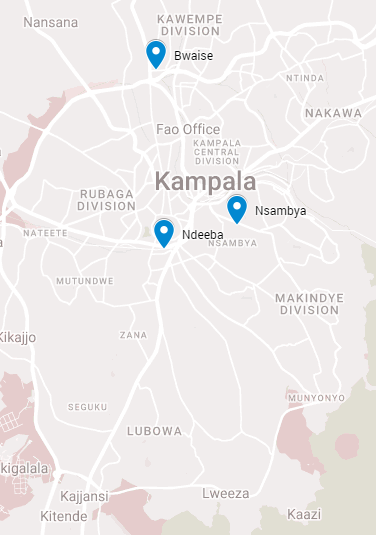
\includegraphics[width=\textwidth]{../../Common/figures/studyArea.png} % Replace with your image path
        \end{column}
        \begin{column}{0.6\textwidth}
            \textbf{1. Study Setting:} Kampala, Uganda
            \begin{itemize}
                \item 23\% urbanized, 60\% semi-urbanized, 17\% rural.
            \end{itemize}
            
            
            \textbf{3. Study Design:}
            \begin{itemize}
                \item Cross-sectional, quantitative.
            \end{itemize}
            
            \textbf{4. Sampling Technique:}
            \begin{itemize}
                \item Probability (random) and non-probability (purposive) sampling.
            \end{itemize}
            
            \textbf{5. Sampling Design:}
            \begin{itemize}
                \item Areas: 
            \end{itemize}
        \end{column}
    \end{columns}
\end{frame}
    
    
    


    \begin{frame}[shrink=20]
        \frametitle{Methodology (2/2)}
        \textbf{6. Sample Size Calculation:}
        \begin{itemize}
            \item Kish-Leslie formula: 50\% prevalence, 95\% confidence, 5\% margin of error.
        \end{itemize}
        
        \textbf{7. Data Collection:}
        \begin{itemize}
            \item Tools: Questionnaire, interviews, visual assessments.
            \item Pretest: 5 participants.
        \end{itemize}
        
        \textbf{8. Quality Control:}
        \begin{itemize}
            \item Pretesting tools, verifying data accuracy.
        \end{itemize}
        
        \textbf{9. Data Analysis:}
        \begin{itemize}
            \item Tools: Microsoft Excel for data summarization.
        \end{itemize}
        
        \textbf{10. Dissemination:}
        \begin{itemize}
            \item Reports to 
        \end{itemize}
\end{frame}
        
    




% \section{Results}

\subsection{Socio-Demographic Characteristics of Respondents}

\begin{frame}{Socio-Demographic Characteristics}

\end{frame}


\subsection{Prevalence of Eye Diseases and Injuries}

\begin{frame}{Eye Injuries \& Diseases (1/2)}

    \begin{figure}
        \centering
        \resizebox{\textwidth}{!}{
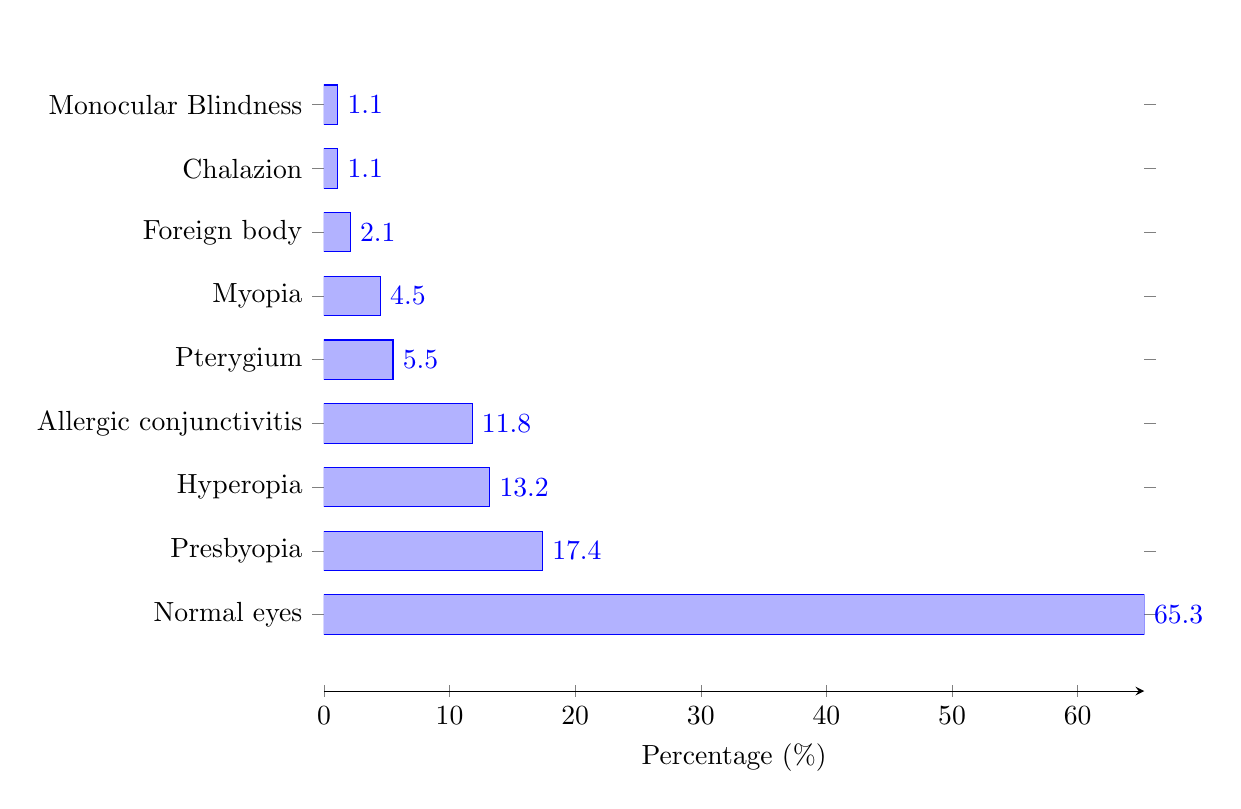
\begin{tikzpicture}
\begin{axis}[
    xbar,
    width=12cm, % Adjust the width to fit your needs
    height=10cm, % Adjust the height to fit your needs
    xlabel={Percentage (\%)},
    symbolic y coords={Normal eyes, Presbyopia, Hyperopia, Allergic conjunctivitis, Pterygium, Myopia, Foreign body, Chalazion, Monocular Blindness},
    ytick=data,
    nodes near coords,
    nodes near coords align={horizontal},
    xmin=0, % Start x-axis from 0
    bar width=0.5cm, % Adjust the bar thickness
    y axis line style={opacity=0},
    axis x line=bottom,
    enlarge y limits=0.15,
]

\addplot coordinates {(65.3,Normal eyes) (17.4,Presbyopia) (13.2,Hyperopia) (11.8,Allergic conjunctivitis) (5.5,Pterygium) (4.5,Myopia) (2.1,Foreign body) (1.1,Chalazion) (1.1,Monocular Blindness)};

\end{axis}
\end{tikzpicture}

}
        \caption{Common Eye Diseases}
    \end{figure}
    

\end{frame}



\subsection{Predisposing Factors for Eye Diseases}


\begin{frame}[shrink=35]{Predisposing Factors \& Use of PED}
    \begin{multicols}{2}
        \begin{table}[h]
    \centering
    \caption{Predisposing Factors (n=232)}
    \scalebox{0.8}{
    \begin{tabular}{lrr}
        \toprule
        \textbf{Factor} & \textbf{Frequency} & \textbf{Percentage (\%)} \\
        \midrule
                \rowcolor{lightblue} % Highlight with light blue
                Working 7 days/week & 146 & 62.9 \\
                \rowcolor{lightblue} % Highlight with light blue
                Working 11-13 hours/day & 118 & 50.9 \\
        PED usage & 105 & 45.3 \\
                \rowcolor{lightblue} % Highlight with light blue
                Not using PED & 127 & 54.7 \\
        \bottomrule
    \end{tabular}}
\end{table}

        \begin{table}[h]
    \centering
    \caption{Reasons for Using PED (n=105)}
    \scalebox{0.85}{
    \begin{tabular}{lrr}
        \toprule
        \textbf{Reason} & \textbf{Frequency} & \textbf{Percentage (\%)} \\
        \midrule
                    \rowcolor{lightblue} % Highlight with light blue
                    Gives protection & 94 & 89.5 \\
        Always available & 6 & 5.7 \\
        Required(authorities) & 4 & 3.8 \\
        \bottomrule
    \end{tabular}}
    \end{table}

    \end{multicols}

\end{frame}



% \note[itemize]{
% \item point 1
% \item point 2
% }

% \section{Discussion}
\begin{frame}
\frametitle{Overview \& Common Eye Conditions}
    \begin{itemize}
        \item \textbf{Prevalence:} 5.5\%, linked to UV radiation, dust, wind, and chemicals \parencite{modenese2018occupational}.
    \end{itemize}
\end{frame}

\begin{frame}
    \frametitle{Eye Injuries \& Impact on Work Performance}
    \begin{itemize}
        \item \textbf{Prevalence:} 52.98\% reported injuries, higher than 32.6\% in Ethiopia \parencite{gebremeskel2019prevalence}.
        \item \textbf{Chemical Exposure:} 10.67\% of woodworkers had chemical injuries, affecting work performance \parencite{iyiade2012pattern}.
    \end{itemize}
\end{frame}
    
\begin{frame}
    \frametitle{Risk Factors \& Occupational Safety}
    
\end{frame}
        


% \input{../../Common/slidesSections/Conclusion}
% \note[itemize]{
% \item point 1
% \item point 2
% }

\begin{frame}[shrink=30]{References}

    % \footnotesize
    % \scriptsize
    % \tiny
    
    \printbibliography
    
    % \begin{multicols}{2}
    % \printbibliography
    % \end{multicols}

\end{frame}

% \begin{frame}[plain]
    \begin{center}
        {\Huge Thank You!}
        
        \vspace{1cm}
        
        {\LARGE "Is It Right OR Is It Right"}
        
        \vspace{0.5cm}
        
        {\large -- }

        \vspace{1cm}
        
        {\Large Any Questions?}

        \vspace{1cm}

        {\large \href{http://hdl.handle.net/20.500.12281/16159}{\textbf{View Our Research Here}}}
    \end{center}
\end{frame}

% Add more sections and subsections as needed


% \begin{frame}[shrink=60, plain]{Global Standards for Protective Eyewear}
    
    \begin{columns}
        \column{0.5\textwidth}
        \begin{figure}
            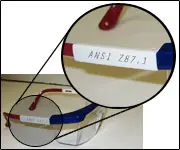
\includegraphics[width=.6\textwidth]{images/Eyewear_pop-out_01-ezgif.com-webp-to-png-converter.png} % Replace with your image path
            \caption{Marker that indicates that the \gls{ped} meets an specifications standard}
        \end{figure}
        
        \textbf{International Standards}
        \begin{itemize}
            \item ISO 12312-1:2013 - Eye and face protection — Sunglasses and related eyewear.
            \item ISO 16321-1:2022 - Eye and face protection for occupational use — General requirements.
            \item ISO 8980-3:2023 - Ophthalmic optics — Uncut finished spectacle lenses.
        \end{itemize}
    
        \textbf{United States}
        \begin{itemize}
            \item ANSI Z87.1-2020 - Occupational and Educational Personal Eye and Face Protection Devices.
            \item OSHA 29 CFR 1910.133 - Standards for eye and face protection in the workplace.
            \item FDA 21 CFR 801.410 - Impact-resistant lenses in eyeglasses and sunglasses.
        \end{itemize}
    
        \textbf{European Union}
        \begin{itemize}
            \item EN 166:2001 - Personal eye-protection specifications.
            \item EN 170:2002 - UV filters for industrial eye protection.
            \item EN 172:1994 - Sunglare filters for industrial use.
        \end{itemize}
    
        \column{0.5\textwidth}
        \textbf{Australia/New Zealand}
        \begin{itemize}
            \item AS/NZS 1337.1:2010 - Eye and face protectors for occupational applications.
            \item AS/NZS 1067.1:2016 - Sunglasses and fashion spectacles.
        \end{itemize}
    
        \textbf{Canada}
        \begin{itemize}
            \item CSA Z94.3-2020 - Eye and face protectors for industrial and other applications.
            \item CAN/CSA-Z94.3.1-16 - Protective eyewear for sports and recreational activities.
        \end{itemize}
    
        \textbf{Japan}
        \begin{itemize}
            \item JIS T 8147:2010 - Eye protection for laser use.
            \item JIS T 8141:2020 - Personal eye-protection equipment.
        \end{itemize}
    
        \textbf{China}
        \begin{itemize}
            \item GB 14866-2006 - National standard for protective eyewear.
            \item GB/T 38120-2019 - General technical requirements for protective eyewear.
        \end{itemize}
    
        \textbf{India}
        \begin{itemize}
            \item IS 5983:1980 - Eye protectors for industrial use.
            \item BIS IS 5983:2018 - Personal eye protection specifications.
        \end{itemize}
    
        \textbf{South Africa}
        \begin{itemize}
            \item SANS 1404:2020 - Eye and face protection.
        \end{itemize}
    
        \textbf{Brazil}
        \begin{itemize}
            \item ABNT NBR 9737:2016 - Eye and face protection for industrial and general use.
        \end{itemize}
    \end{columns}
    \end{frame}
    


% \begin{frame}[plain, shrink=25]{Occupational Safety and Health Act 9, 2006 and Eye Health}
    \begin{multicols}{2}

        \begin{itemize}
            \item \textbf{Introduction to the OSH Act:}
            \begin{itemize}
                \item The OSH Act 9, 2006 provides a legal framework for workplace safety and health.
                \item Eye health is a critical aspect protected under this Act.
            \end{itemize}
            
            \item \textbf{Relevant Sections for Eye Health:}
            \begin{itemize}
                \item \textbf{Section 92 - Protection of Eyes:} 
                \begin{itemize}
                    \item Mandates provision of protective eyewear for hazardous processes.
                \end{itemize}
                \item \textbf{Section 13 - Training Requirements:} 
                \begin{itemize}
                    \item Employees must be trained on proper use of protective equipment.
                \end{itemize}
                \item \textbf{Section 35 - Duties of Employees:} 
                \begin{itemize}
                    \item Employees must use protective equipment properly and responsibly.
                \end{itemize}
            \end{itemize}
    
            \item \textbf{Case Studies:}
            \begin{itemize}
                \item Examples of workplace incidents where non-compliance led to eye injuries.
            \end{itemize}
            
            \item \textbf{Compliance and Best Practices:}
            \begin{itemize}
                \item Employers should ensure compliance to protect eye health.
                \item Regular inspections and maintenance of protective gear are essential.
            \end{itemize}
            
            \item \textbf{Conclusion:}
            \begin{itemize}
                \item Reiterate legal obligations and the moral duty to protect employee vision.
            \end{itemize}
        \end{itemize}

    \end{multicols}
        

\end{frame}



\end{document}